\documentclass[serif,8pt]{beamer}
\usetheme{default} % You can change the theme here
\usecolortheme{metropolis} % You can change the color theme here

% Packages for additional functionality
\usepackage{graphicx} % For including images
\usepackage{amsmath} % For mathematical symbols and equations
\usepackage{multirow}
\usepackage{subfig}
\usepackage{braket}
\usepackage{caption}
% \usepackage{authblk}

% /home/bogfootlj/.local/share/fonts/NerdFonts
% Setting up fonts

\graphicspath{{./Images/}} % Where to take images from
\setbeamertemplate{section in toc}[sections numbered]
\setbeamertemplate{subsection in toc}[subsections numbered]

\captionsetup[figure]{labelformat=empty}% redefines the caption setup of the figures environment in the beamer class.
\captionsetup[table]{labelformat=empty}% redefines the caption setup of the figures environment in the beamer class.

% Define the style for the footer with page numbers
\setbeamercolor{footline}{fg=black}

% Define a command to exclude the page counter from the first two slides
\newcommand{\noPageNumber}{%
    \setbeamertemplate{footline}{}%
}

% Define a command to reset the page counter and start numbering from the third slide
\newcommand{\resetPageNumber}{%
    \setbeamertemplate{footline}{%
        \begin{beamercolorbox}[wd=\paperwidth,ht=0.5ex,dp=1ex]{foot}%
            \hspace*{1em}\hfill \insertframenumber/\inserttotalframenumber\hspace*{1em}%
        \end{beamercolorbox}%
    }%
    \addtocounter{framenumber}{-2}
}

% Set up the footer for the rest of the presentation
\setbeamertemplate{footline}{%
    \begin{beamercolorbox}[wd=\paperwidth,ht=0.5ex,dp=1ex]{foot}%
        \hspace*{1em}\hfill%
        \insertframenumber/\inserttotalframenumber\hspace*{1em}%
    \end{beamercolorbox}%
}


% Title slide information
\title{Generating and teleporting entanglement for quantum networks}
\author[Adrian, Rainer]{Adrian Udovičić\\\and Assoc. prof. dr. Rainer Kaltenbaek}
\institute{University of Ljubljana, Faculty of Mathematics and Physics}
\date{23.05.2024, Ljubljana, Slovenia}
\logo{
\includegraphics[height=1cm]{CombinedLogo.png}}

\begin{document}
% Local background must be enclosed by curly braces for grouping.
{\setbeamertemplate{footline}{}}
\usebackgroundtemplate{\includegraphics[width=\paperwidth,height=\paperheight]{~/Notes/PhDNotes/PhDTopicDefenseAbstract/Seminar/Presentation/Images/SagnacWithSomeAddedColoursV3.png}}
\noPageNumber
\begin{frame}
	\titlepage
\end{frame}

\usebackgroundtemplate{}
\noPageNumber
\begin{frame}{Contents and introduction}
  \tableofcontents % Include a table of contents slide
\end{frame}

\resetPageNumber

\section{Motivation}
\begin{frame}{Motivation}
	\begin{minipage}[l]{0.48\textwidth}
		\begin{itemize}
			\item SiQUID 
				\begin{enumerate}
					\item[0.] Proof of concept
					\item Entanglement distribution
					\item Entanglement based Quantum Key Distribution (QKD)
					\item Training in quantum technologies in Slovenia
					\item Testbed for industrialized version
				\end{enumerate}
		\end{itemize}
	\end{minipage}
	\begin{minipage}[r]{0.48\textwidth}
		\begin{figure}
			\begin{center}
				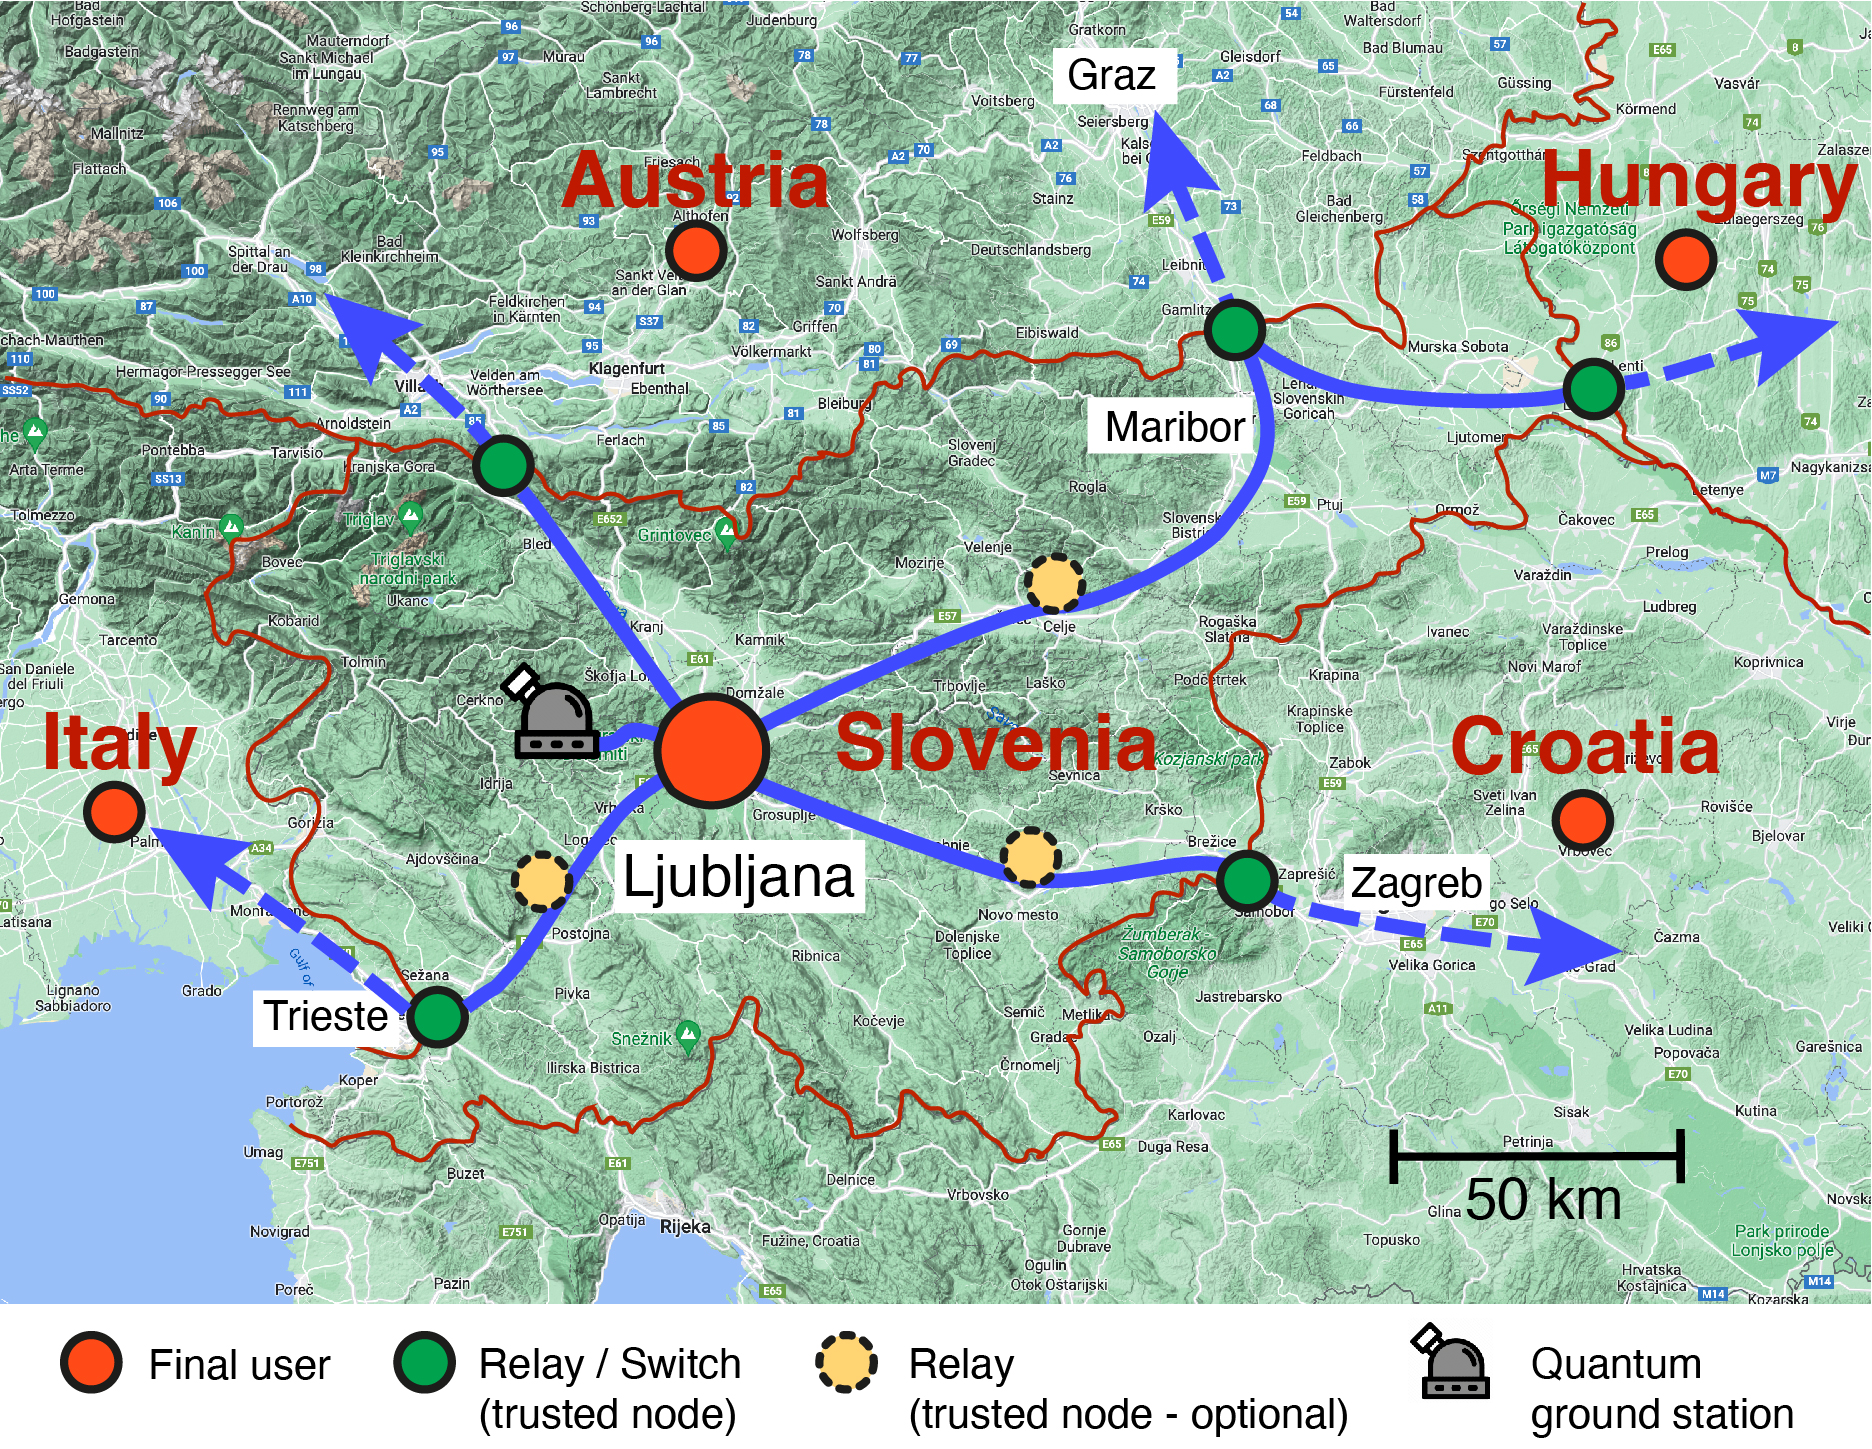
\includegraphics[width=5cm]{SI_network_with_groundstation.jpg}
			\end{center}
			\caption{Example of Slovenian Quantum Network.}
		\end{figure}
	\end{minipage}
\end{frame}

\addtocounter{framenumber}{-1}
\begin{frame}{Motivation}
	\begin{minipage}[l]{0.48\textwidth}
		\begin{itemize}
			\item SiQUID 
				\begin{enumerate}
					\item[0.] Proof of concept
					\item Entanglement distribution
					\item Entanglement based Quantum Key Distribution (QKD)
					\item Training in quantum technologies in Slovenia
					\item Testbed for industrialized version
				\end{enumerate}
			\item Bright source of entanglement
		\end{itemize}
	\end{minipage}
	\begin{minipage}[r]{0.48\textwidth}
		\begin{figure}
			\begin{center}
				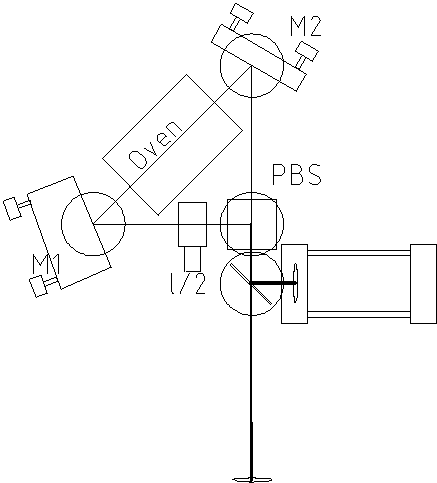
\includegraphics[width=5cm]{SagnacCAD.png}
			\end{center}
			\caption{An example of a Sagnac Interferometer.}
		\end{figure}
	\end{minipage}
\end{frame}

\section{Theory}
\subsection{Spontaneous Parametric Downconversion (SPDC)}

\begin{frame}{SPDC}
	\framesubtitle{Spontaneous Parametric Downconversion (SPDC)}
	\begin{minipage}[l]{0.60\textwidth}
		\begin{figure}
			\begin{center}
				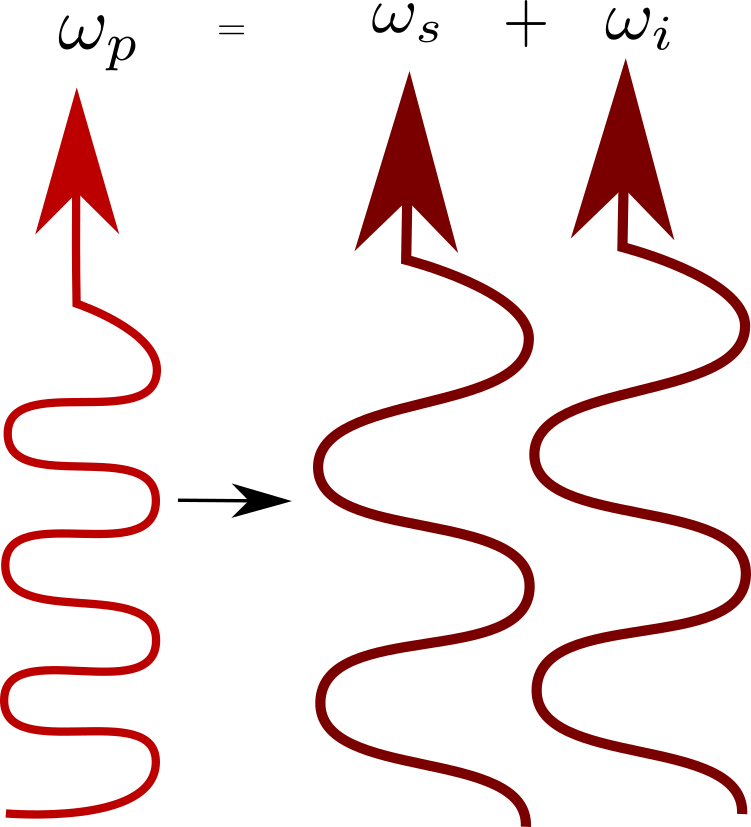
\includegraphics[width=5cm]{SPDC.png}
			\end{center}
			\caption{Illustration of SPDC}
			\label{fig:SPDC}
		\end{figure}
	\end{minipage}
	\begin{minipage}[r]{0.35\textwidth}
		\begin{itemize}
			\item Degenerate $\omega_i = \omega_s$
			\item Non-degenerate $\omega_i \ne \omega_s$
		\end{itemize}
	\end{minipage}
	% What is SPDC used for
\end{frame}

\subsubsection{Phase Matching}

\begin{frame}
	\frametitle{Phase Matching}
	\framesubtitle{Birefringent Phase Matching, Quasi Phase Matching}
\begin{figure}
	What is Phase Matching?
		\begin{center}
		\caption{Illustration of Birifringent Phase Matching $k_p - k_i - k_s = 0$ and}
		  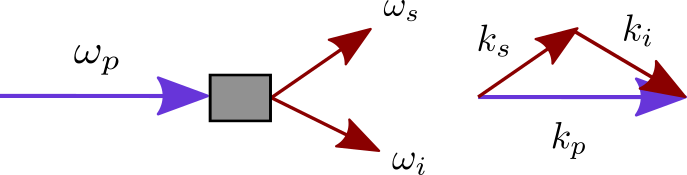
\includegraphics[width=8.5cm]{SPDCkPM.png}\\
		\caption{Quasi Phase Matching $k_p - k_i -k_s - \Delta k = 0$.}
		  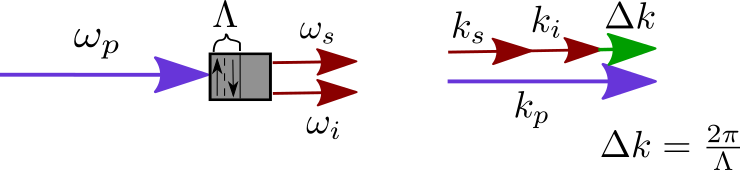
\includegraphics[width=8.5cm]{SPDCkQPM.png}
		\end{center}
		%Conservation of momentum add here noob
		\label{fig:SPDCk}
	\end{figure}
	% \Huge
	% \begin{equation*}
	% 	I &\propto \text{sinc}^2\left(\frac{L \delta k}{2}\right)
	% 	\label{eq:SPDCksinc2}
	% \end{equation*}
\end{frame}


\begin{frame}[t]
	\frametitle{Phase Matching}
	\framesubtitle{Crystal Size}
	\begin{figure}
		\caption{Difference in photon generation between a unpoled and poled crystal.\\\textit{Source: RP-Photonics}}
		\begin{center}
			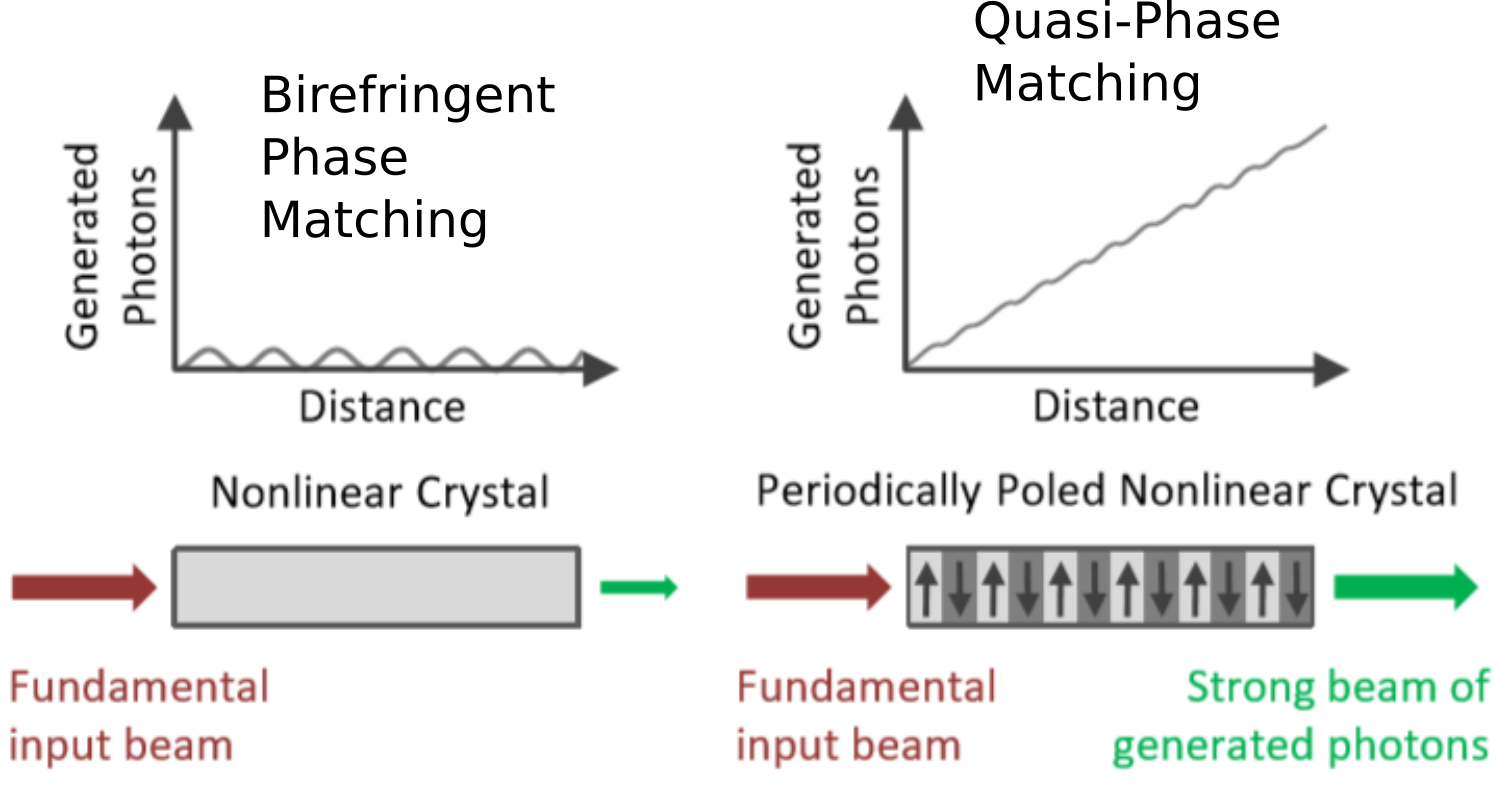
\includegraphics[width=10cm]{PolledVsNot.png}
		\end{center}
		\label{fig:poledvsnot}
	\end{figure}
\end{frame}

\begin{frame}[t]
	\frametitle{Phase Matching}
	\framesubtitle{Types}
	\begin{minipage}[l]{0.35\textwidth}
		\begin{itemize}
			\item Type-0 : o $\rightarrow$ o + o
			\item Type-I : o $\rightarrow$ e + e
			\item Type-II : e $\rightarrow$ e + o
		\end{itemize}
	\end{minipage}
	\begin{minipage}[r]{0.60\textwidth}
		\begin{figure}
			\begin{center}
				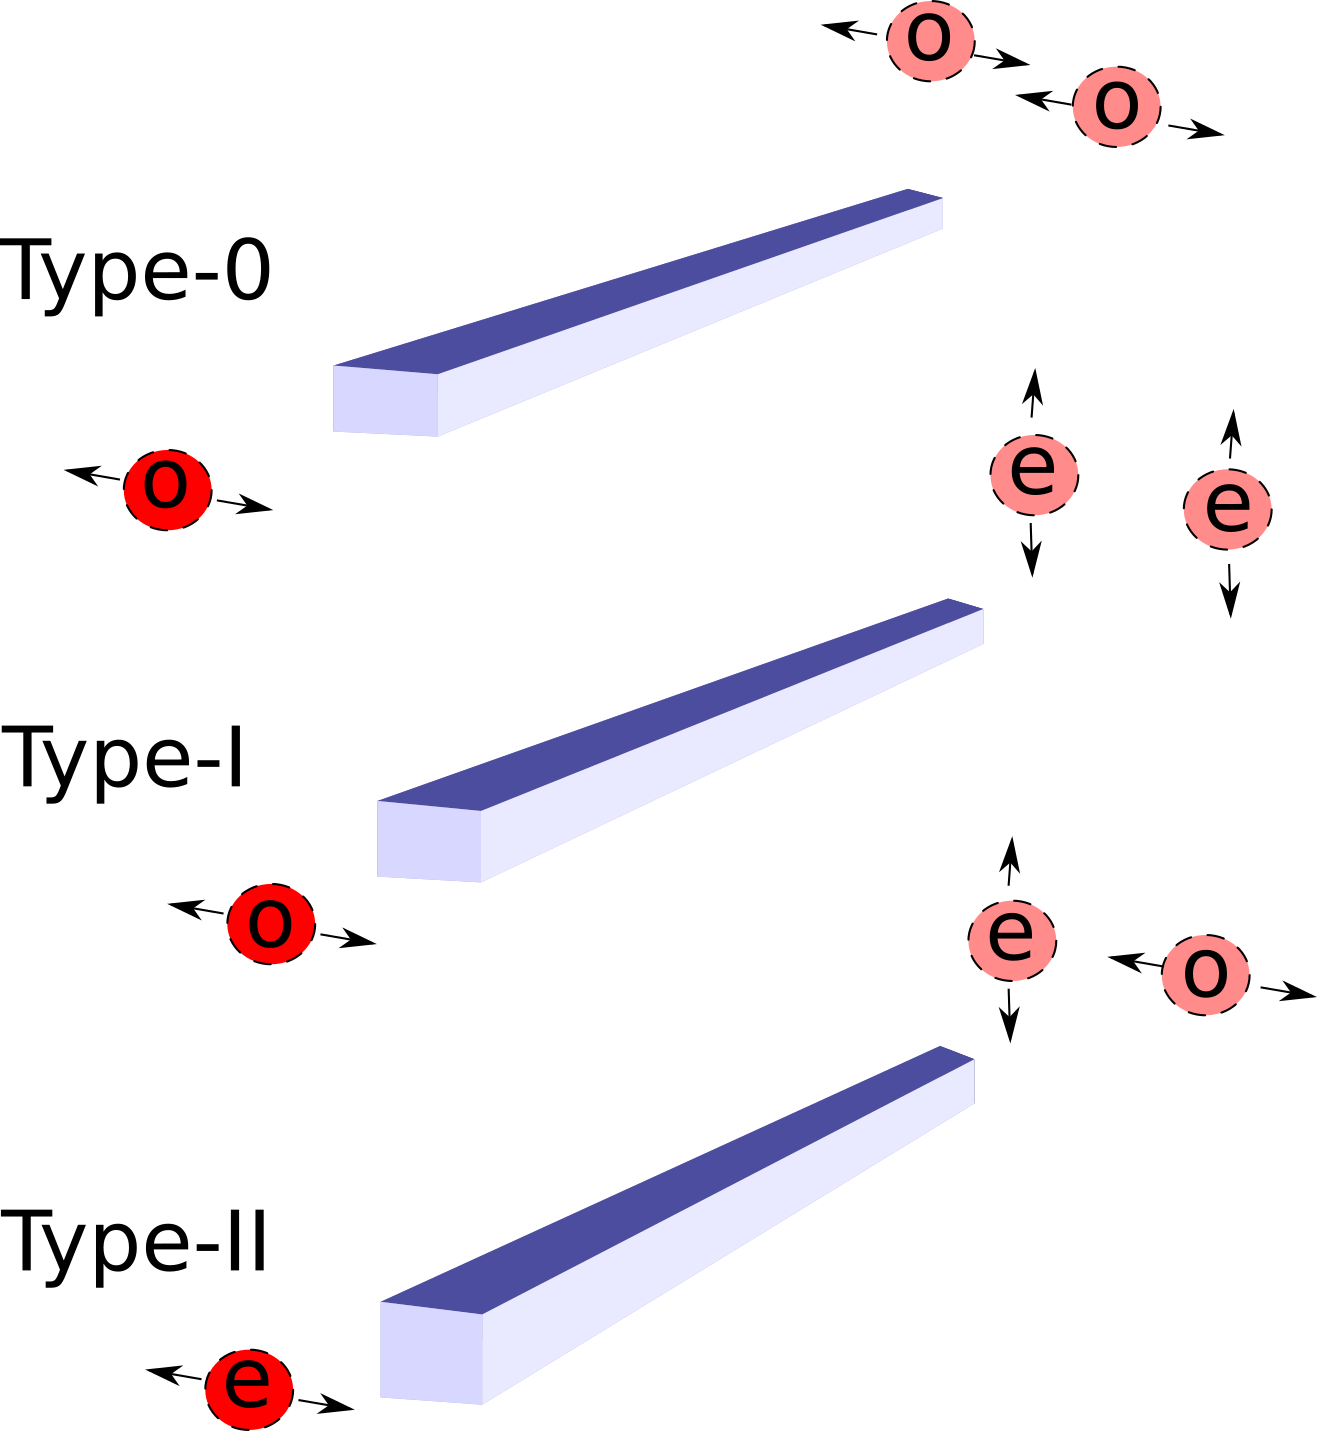
\includegraphics[width=6cm]{TypesOfConversions}
			\end{center}
			\caption{Illustration of different types of polarization conversions.}
		\end{figure}
	\end{minipage}
\end{frame}

\begin{frame}{Phase Matching}
	\framesubtitle{Phase Matching Temperature}
	\begin{figure}[!ht]
	  \centering
	  \caption{Phase Matching Temperature plots for a) Type-2 crystal of 9,12 $\mu$m poling period, b) Type-0, 19,25 $\mu$m, c) Type-0, 19,45 $\mu$m, d), Type-0 19,65 $\mu$m. $\delta \phi = \frac{L \Delta k}{2}$}
	  \subfloat[][]{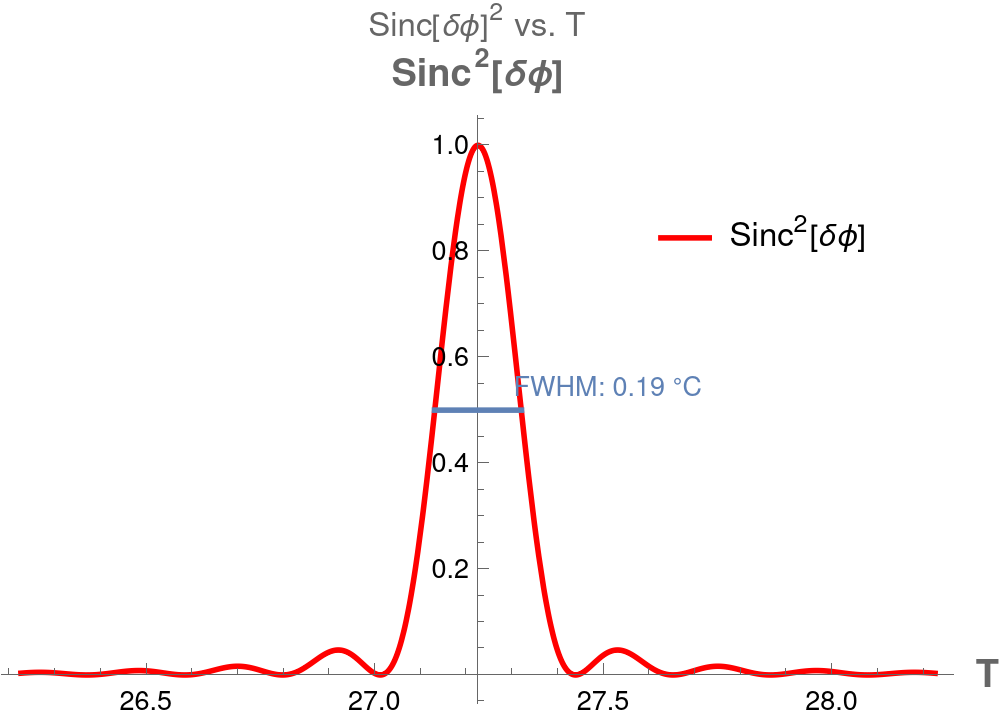
\includegraphics[width=3.9cm]{PMT_Type2.png}}\quad
	  \subfloat[][]{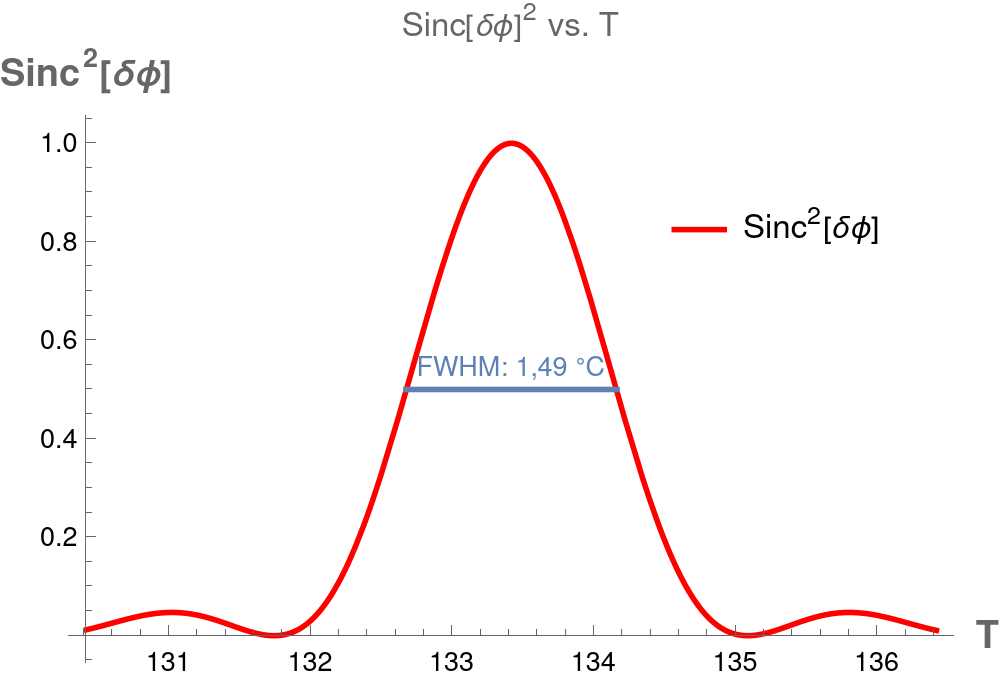
\includegraphics[width=3.9cm]{PMT_Type0G4.png}}\\
	  \subfloat[][]{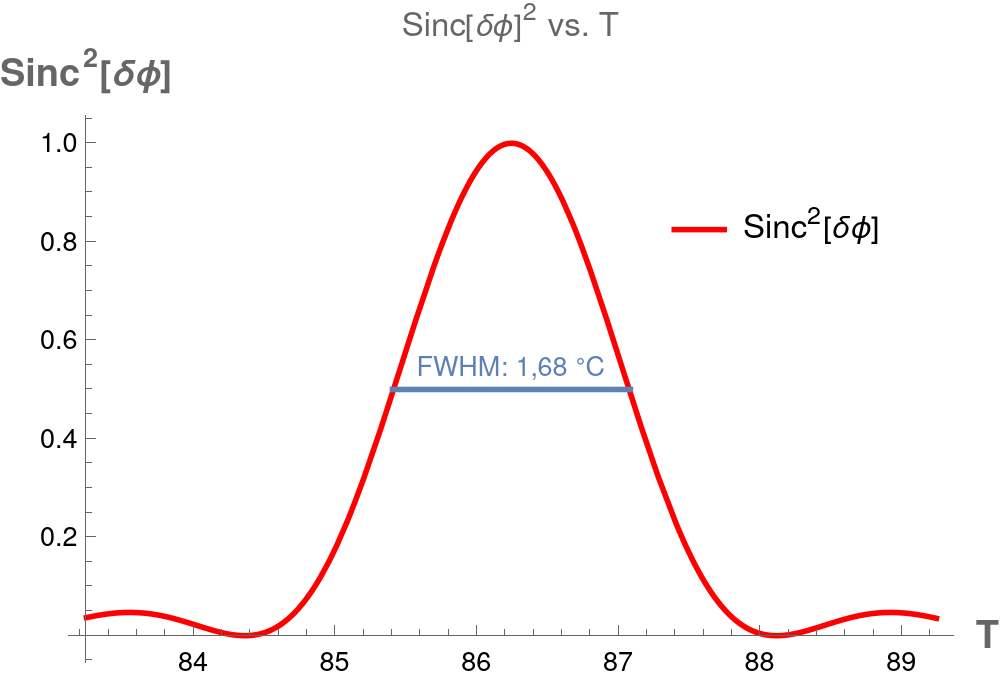
\includegraphics[width=3.9cm]{PMT_Type0G5.png}}\quad
	  \subfloat[][]{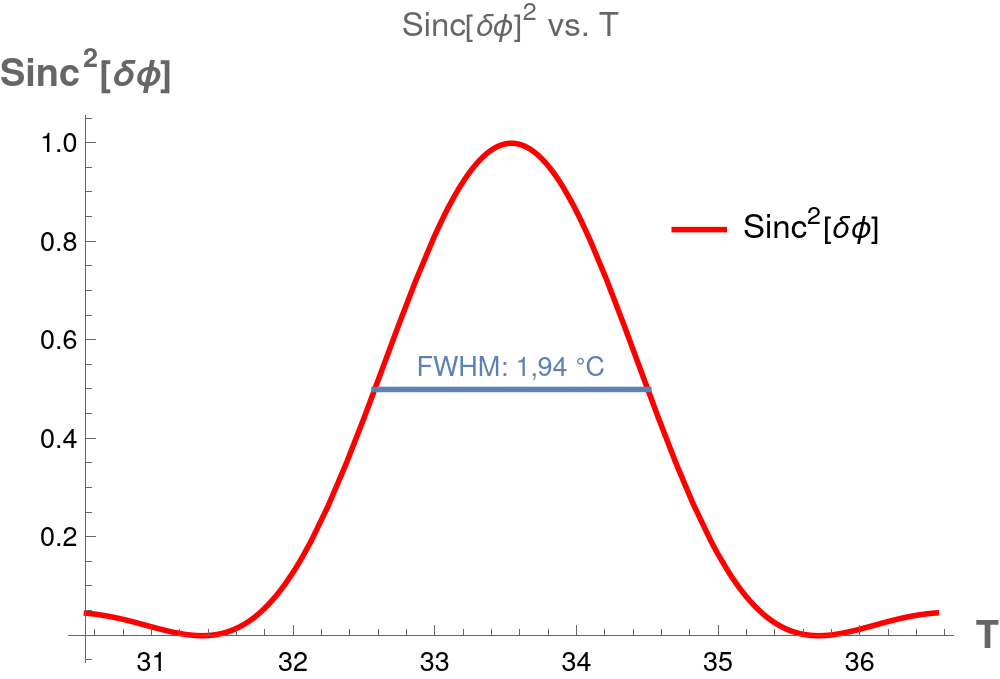
\includegraphics[width=3.9cm]{PMT_Type0G6.png}}\\
	  \label{fig:gratingstheory}
	\end{figure}
\end{frame}

\begin{frame}[t]
	\frametitle{Phase Matching}
	\framesubtitle{Bandwidth}
	\begin{figure}[!ht]
	  \centering
	  \caption{Wavelength bandwidth of a) Type-2 crystal with a poling period of 9,12 $\mu$m\\ b) Type-0 crystals with poling periods of 19,25 $\mu$m}
	  % Do this on the same plot
	  \subfloat[][]{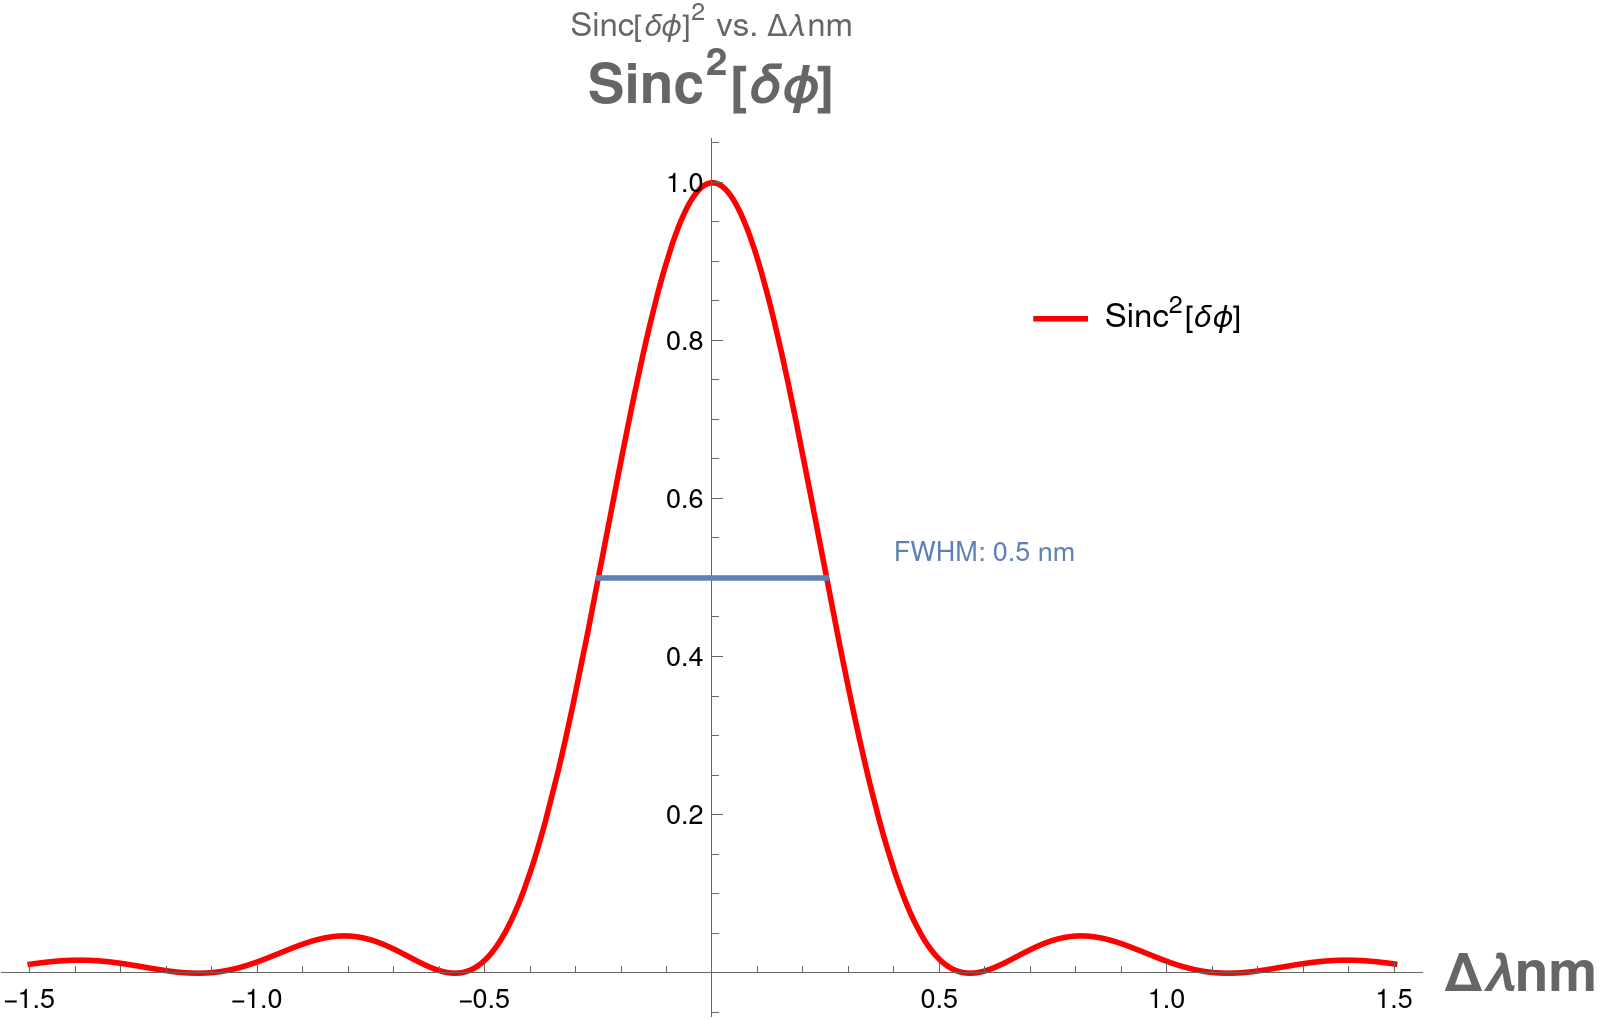
\includegraphics[width=5cm]{Type2wavelength.png}}\quad
	  \subfloat[][]{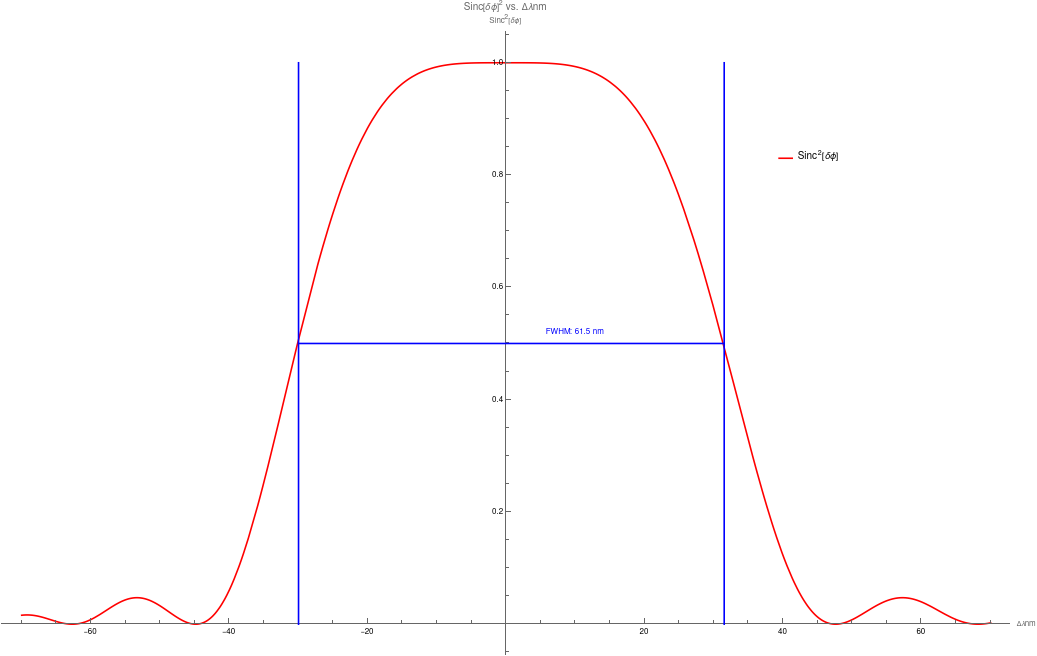
\includegraphics[width=5.5cm]{Type0wavelength.png}}
	  \label{fig:CompT0a2}
	\end{figure}
\end{frame}


\begin{frame}[t]
	\frametitle{Existing sources}
	\framesubtitle{Comparison between different groups}
	\small
\begin{table}
    \caption{Comparison of different sources}\label{SotA}
    \centering
	\begin{tabular}{|c||c|c|c|c|c|}
        \hline
		& & & & & \\ % Empty line for spacing
        \multirow{2}{*}{\shortstack{Who\\When}}& \multirow{2}{*}{\shortstack{\cite{1}\\2022 }} &\multirow{2}{*}{\shortstack{\cite{4}\\2012 }}  &\multirow{2}{*}{\shortstack{\cite{3}\\2007 }}   & \multirow{2}{*}{\shortstack{\cite{2}\\2006 }}  & \multirow{2}{*}{\shortstack{\cite{5}\\2010 }} \\
		& & & & & \\ % Empty line for spacing
		& & & & & \\ % Empty line for spacing
		% add years
		\hline
        \hline
        Type & 0 & 0 & II & II & II  \\
        \hline
		\multirow{2}{*}{\shortstack{Brightness [$\frac{\text{Hz}}{\text{mW nm}}$]}} & \multirow{2}{*}{2,5$\times$$10^6$} & \multirow{2}{*}{0,278$\times$$10^6$} & \multirow{2}{*}{0,273$\times$$10^6$} & \multirow{2}{*}{0.005$\times$$10^6$} & \multirow{2}{*}{0.087$\times$$10^6$}  \\
		& & & & & \\ % Empty line for spacing
        \hline
        Bandwidth [ nm ] & 106 & 2,3 & 0,3 & 1 & 0,3  \\
        \hline
    \end{tabular}
\end{table}
\normalsize
\end{frame}


%	TODO: DO THIS ALREADY YOU IDIOT
% \subsubsection{Efficiency}
% \begin{frame}
% 	\frametitle{SPDC}
% 	\framesubtitle{Expected efficiency}
% 	Fiorentino Expected efficiency
% 	Might not be important
% \end{frame}


%	TODO: DO THIS ALREADY
% \subsubsection{Detectors}
% \begin{frame}
% 	\frametitle{Detectors}
% 	\framesubtitle{Dependence of detector dead-time and efficiency}
% 	\Huge Most important
% 	\large
% Dead-time dependency
% \end{frame}

\begin{frame}[t]
	\frametitle{Different Designs}
	\begin{figure}[!ht]
	  \centering
	  \caption{Different design ideas from other groups. a) \cite{design4}, b) \cite{design1}, c) \cite{design3}, d) \cite{design2}}
	  \subfloat[][]{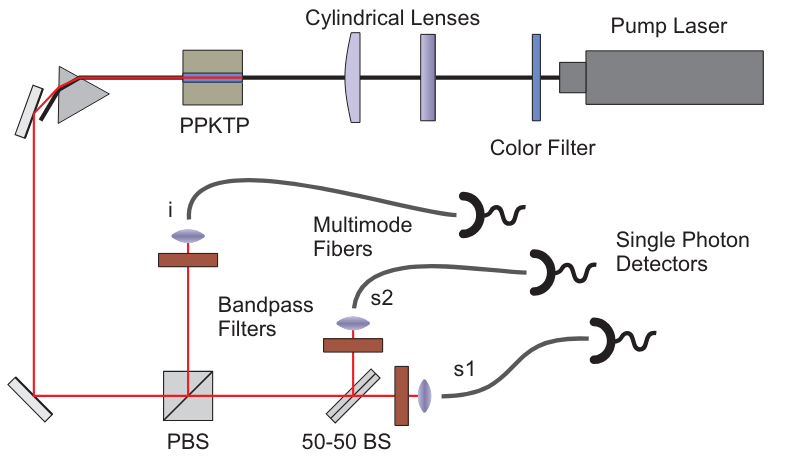
\includegraphics[width=5cm]{Design4.png}}\quad
	  \subfloat[][]{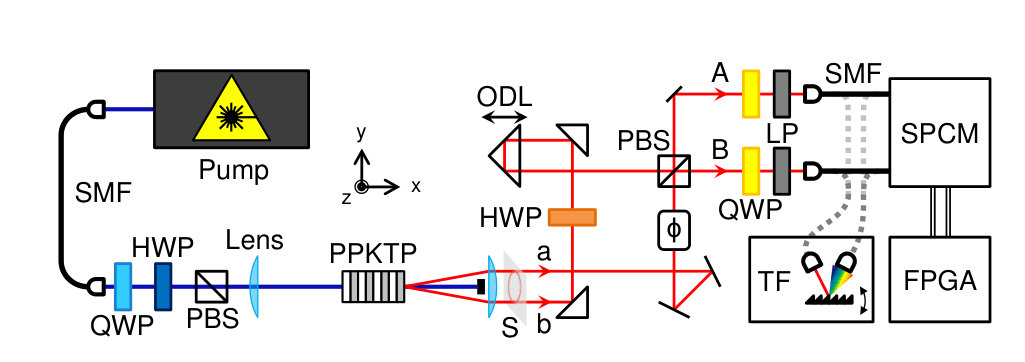
\includegraphics[width=5cm]{Design1.png}}\\
	  \subfloat[][]{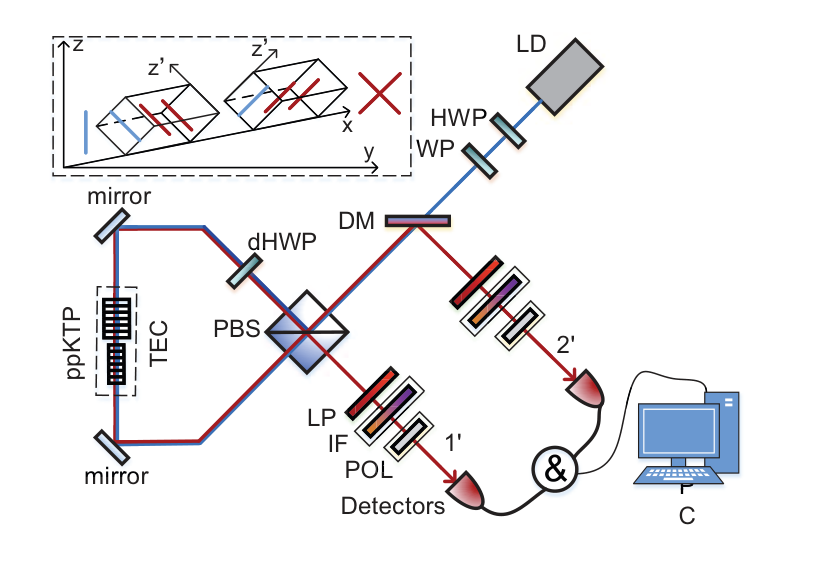
\includegraphics[width=4cm]{Design3.png}}\quad
	  \subfloat[][]{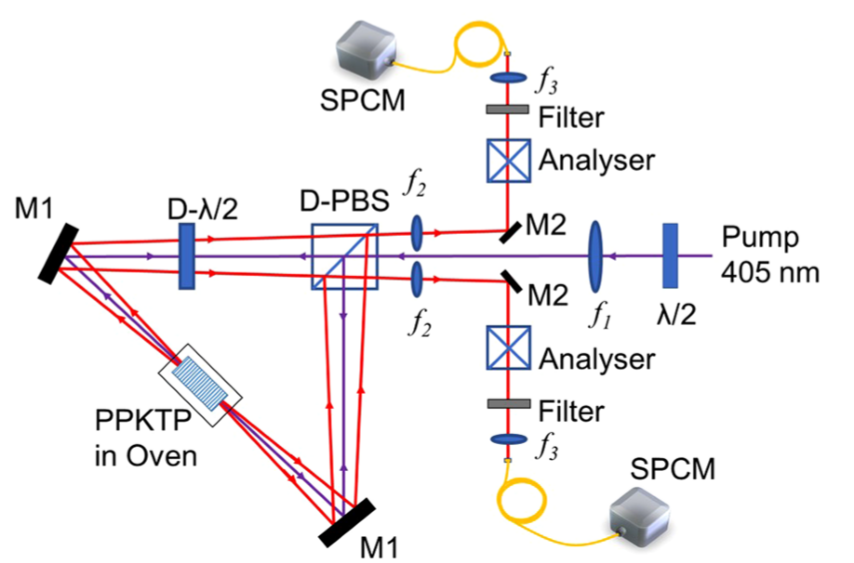
\includegraphics[width=4.5cm]{Design2.png}}\\
	  \label{fig:sub4}
	\end{figure}
\end{frame}

\subsection{Distributing Entanglement}
\begin{frame}{Distributing Entanglement}
	\framesubtitle{Introduction}
	% Making source of these entangled states.
	% \begin{equation*}
	% 		\ket{\Psi_{p}} = \frac{1}{\sqrt{2}} ( a_{H}^{\dagger} ( \omega_p ) + a_{V}^{\dagger} ( \omega_p ) )\ket{0}\\
	% \end{equation*}
	\begin{minipage}[l]{0.48\textwidth}
		\begin{equation*}
		\begin{aligned}
			\ket{\Psi_{\text{Type-2}}} &= \frac{1}{\sqrt{2}}(a_{H}^{\dagger}(\omega_s)a_{V}^{\dagger}(\omega_i)+\\
								&a_{V}^{\dagger}(\omega_i)a_{H}^{\dagger}(\omega_s))\ket{0}\\
		\end{aligned}
		\end{equation*}
	\end{minipage}
	\begin{minipage}[r]{0.48\textwidth}
	\begin{equation*}
		\begin{aligned}
			\ket{\Psi_{\text{Type-0}}} &= \frac{1}{\sqrt{2}}(a_{H}^{\dagger}(\omega_s)a_{H}^{\dagger}(\omega_i)+\\
									   &a_{V}^{\dagger}(\omega_i)a_{V}^{\dagger}(\omega_s))\ket{0}
		\end{aligned}
	\end{equation*}
	\end{minipage}
	\begin{itemize}
			%	DONE TODO: Make a graphic of this
			%	Two pairs of maximally entangled qubits.
			%	Pair one = qubit 1 and qubit 2
			%	Pair two = qubit 3 and qubit 4
			%	Teleport qubit 2: Perform Bell State Measurement on qubit 2 and qubit 3
			%	If teleportation + success == true -> qubit 2 and qubit 3 states are destroyed (no-cloning theorem) -> Qubit 1 and Qubit 4 now in same entangled state
			% NOTE: Distillation and repeaters - Rainer PhD ----
		\item FMF/IJS
		\item Nodes in Ljubljana % - Entanglement distribution
	\end{itemize}
\end{frame}

\begin{frame}[t]
	\frametitle{Entanglement}
	\framesubtitle{What is it good for?}
	\begin{itemize}
		\item Entanglement source applications:
			\begin{enumerate}
				\item Distributed Quantum Computation - Send a state then receive a result on the entangled pair,
				% \item Quantum Algorithms,
				% \item Quantum Metrology, % Part of quantum sensing
				\item Quantum Sensing,
				% \item Entanglemenet swapping,
				\item Single Photon Source - Calibration
			\end{enumerate}
		\item Loss in fiber $\rightarrow$ Entanglement swapping!
	\begin{table}
		\caption{Relevant fiber loss. \textit{Source: \href{https://www.thorlabs.com/newgrouppage9.cfm?objectgroup_id=949}{Thorlabs}}}
		\label{tab:fiberloss}
		\begin{tabular}{|c|c|c|c|c|c|c|}
			\hline
			$\lambda$ [nm] & 430 & 532 & 780 & 1310 & 1550 & 1900\\
			\hline
			Loss [dB/km] & 50 & 30 & 12 & 0.32 &  0.18 & 5\\
			\hline
		\end{tabular}
	\end{table}
	\begin{figure}
		\begin{center}
			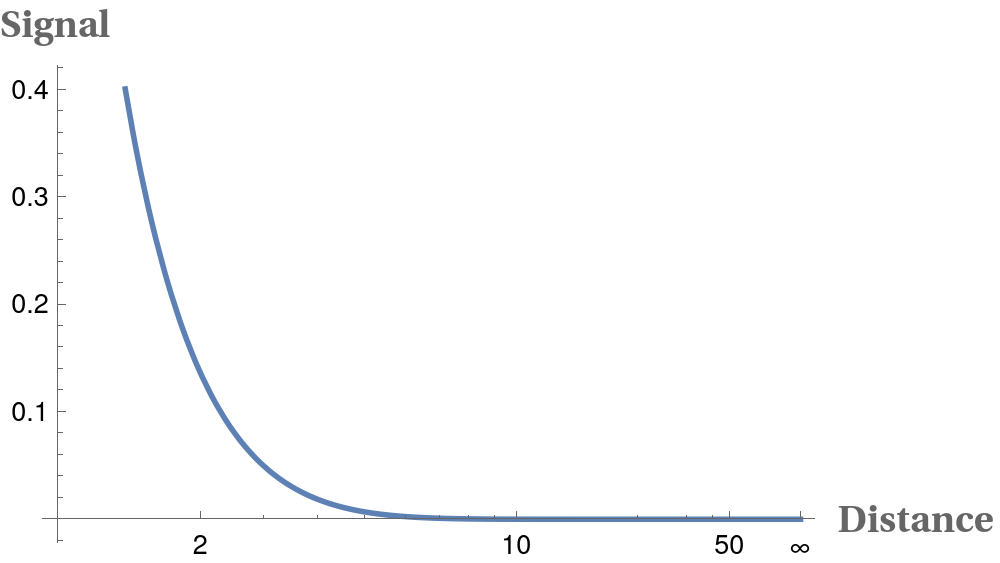
\includegraphics[width=6cm]{FiberLoss.png}
		\end{center}
		\caption{Loss in fiber over distance.}\label{fig:fiberloss}
	\end{figure}
	\end{itemize}
\end{frame}



\subsubsection{Quantum Teleportation}
\begin{frame}[t]
    \frametitle{Distributing entanglement}
    \framesubtitle{Teleportation}
    \begin{figure}[]
      \centering
      \caption{Illustration of Quantum Teleportation: Basis of Entanglement Swapping.}
      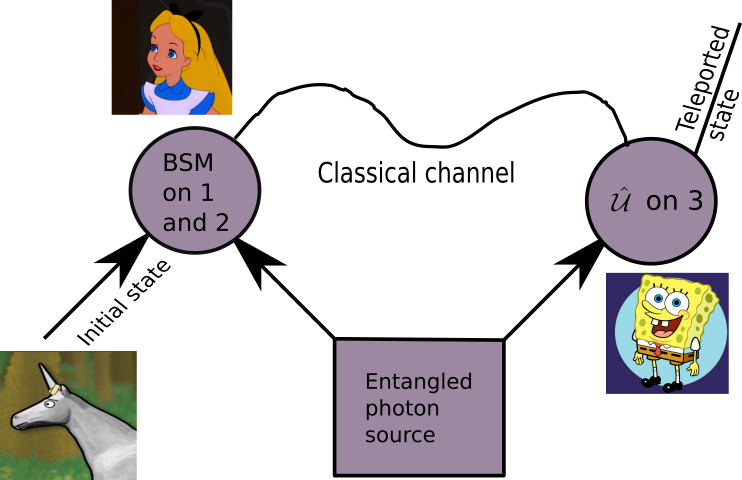
\includegraphics[width=8cm]{EntanglementTeleportation.png}
	\label{fig:Tele}
    \end{figure}
\end{frame}

%add image for the 50% case -> PBS after BS
\begin{frame}[t]
	\frametitle{Entanglement Distribution}
	\framesubtitle{Bell State Measurement}
	\begin{figure}
		\begin{center}
			\subfloat[][]{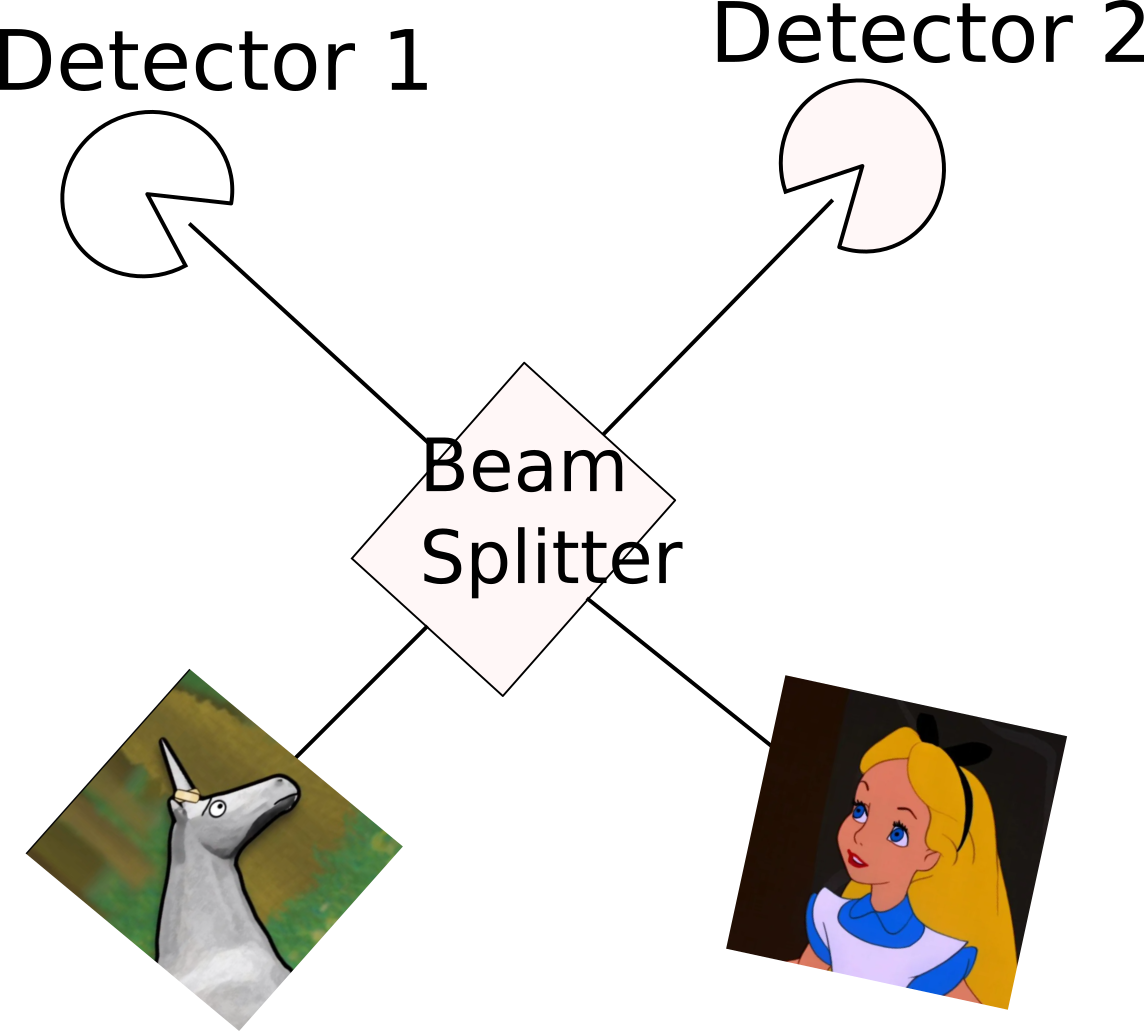
\includegraphics[width=5cm]{BSM.png}}\quad
			\subfloat[][]{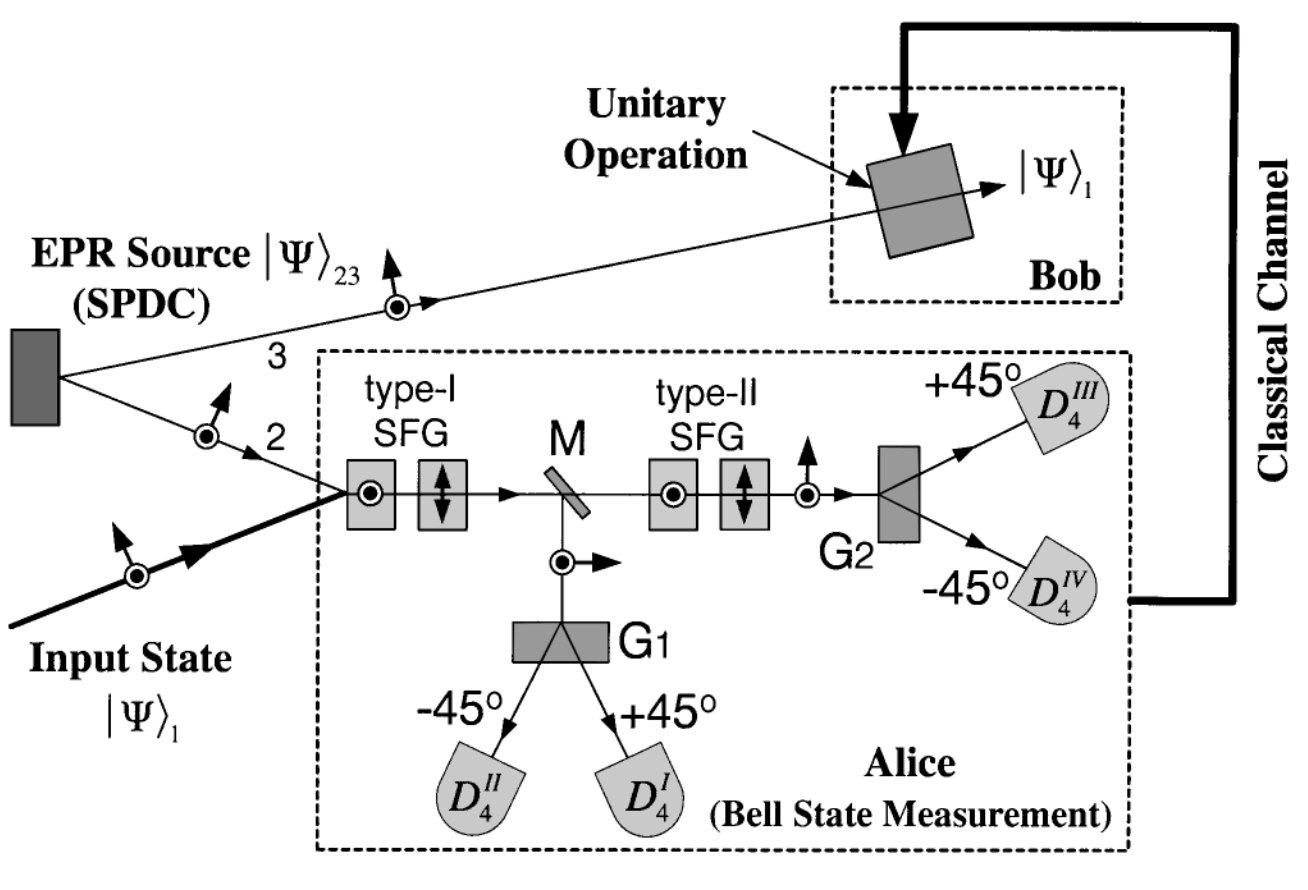
\includegraphics[width=5cm]{FullBSM.png}}\\
		\end{center}
		\caption{The simplest and the not so simple Bell State Measurement.}
		\label{fig:BSMSimple}
	\end{figure}
\end{frame}


\subsubsection{Entanglement Swapping}
\begin{frame}[t]
    \frametitle{Distributing entanglement}
    \framesubtitle{Swapping}
\begin{figure}[]
      \centering
      \caption{Illustration of Entanglement Swapping: Prerequisite for a Quantum Repeater.}
      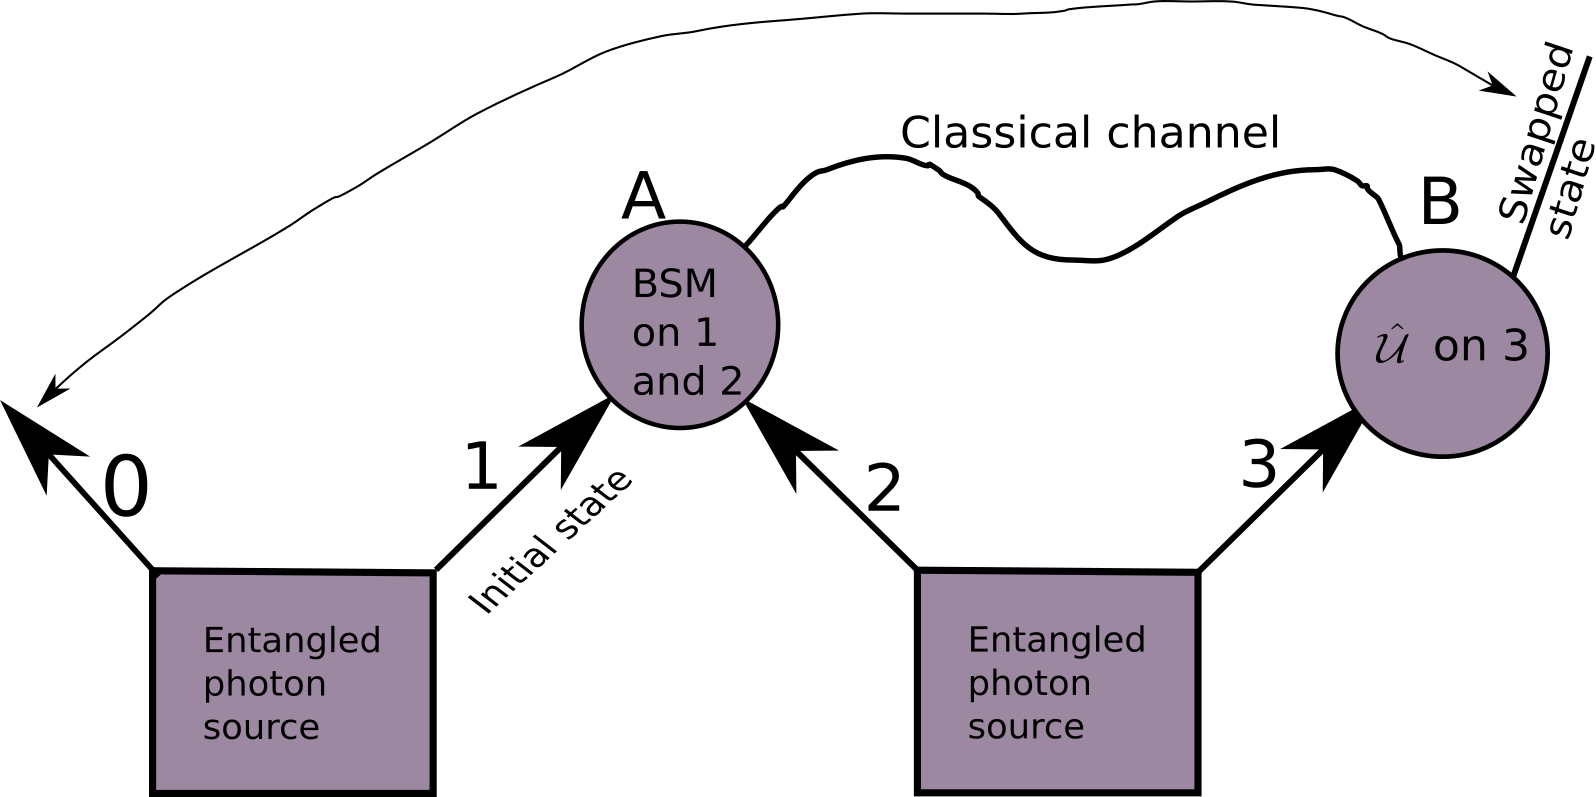
\includegraphics[width=10cm]{EntanglementSwapping.png}
	\label{fig:Swap}
    \end{figure}
		% 	QUANTUM REPEATERS IN HANDWAVEY WAY
\end{frame}

\begin{frame}[t]{Possible realization of the Slovenian Network}
	\begin{figure}
		\begin{center}
			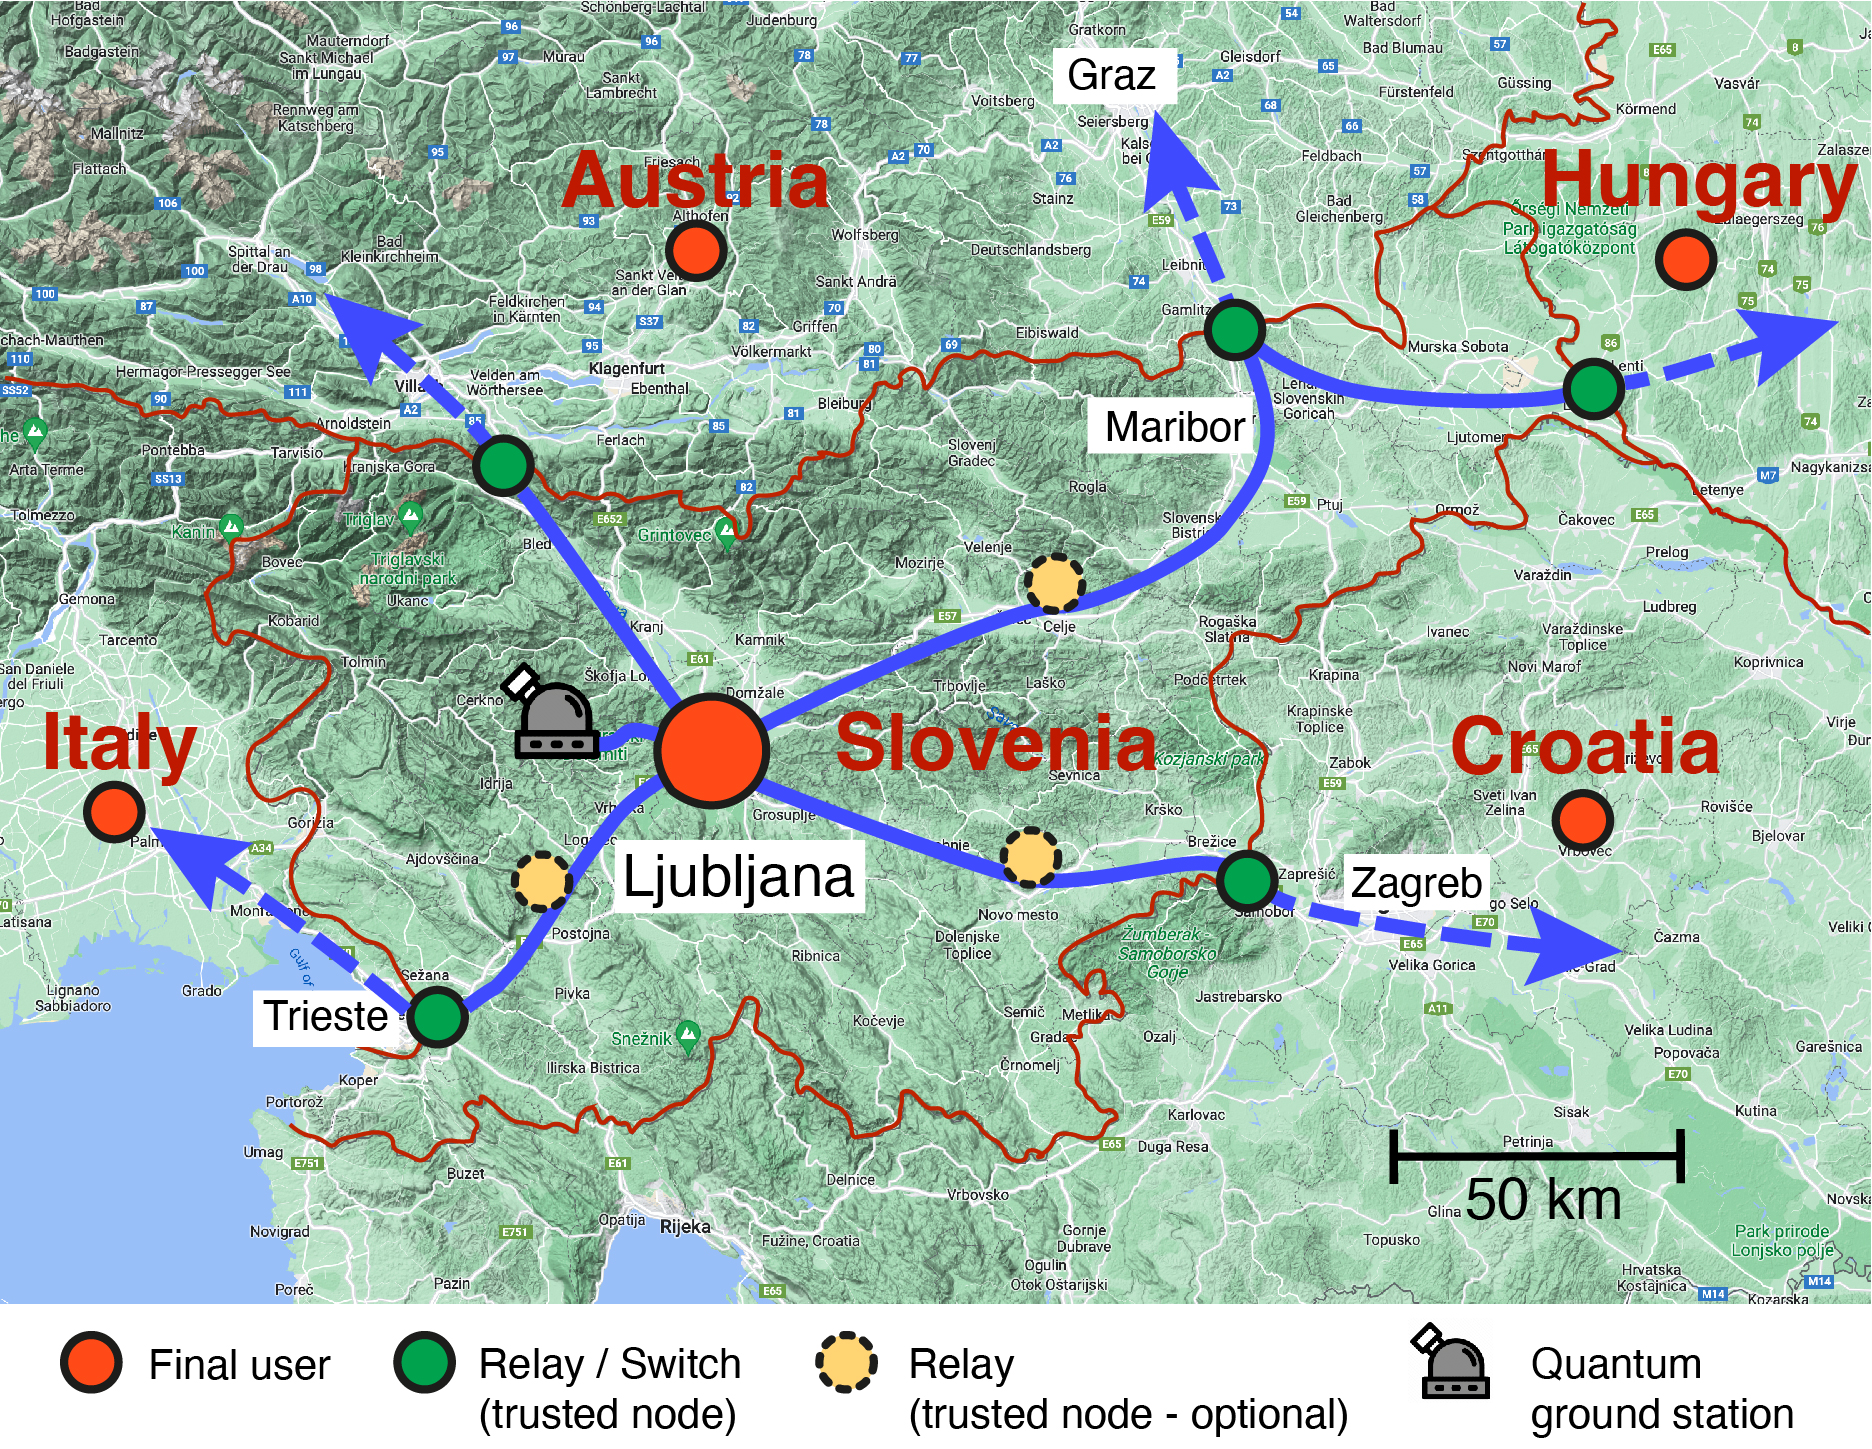
\includegraphics[width=0.9\textwidth]{SI_network_with_groundstation.jpg}
		\end{center}
		\caption{Example of the Slovenian Quantum Network.\\\textit{Source: \url{https://siquid.fmf.uni-lj.si/}.}}
	\end{figure}
\end{frame}

\section{Present state}
\subsection{Parameters}
\begin{frame}[t]
	\frametitle{Present state}
	\framesubtitle{Parameters}
		\begin{itemize}
			\item Focusing parameters \cite{bennik}
					\begin{equation*}
							\xi = \frac{L}{2 z_R} = 2.08
						\label{eq:Focusing parameter}
					\end{equation*}\\
			\item Correct lenses and distances for efficient coupling
		\end{itemize}
	\begin{figure}[!ht]
	  \centering
	  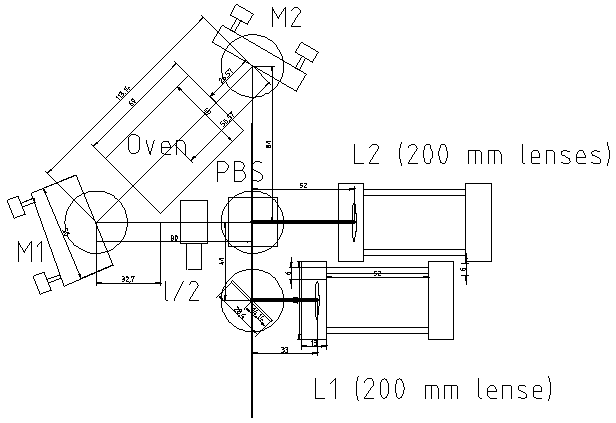
\includegraphics[width=6cm]{SagnacDesign.png}
	  \caption{Design of the Sagnac interferometer.}
	\end{figure}
\end{frame}

\subsection{Phase Matching Temperature}
%Temperatures in the 100°C-200°C range are used in order to minimize the photorefractive effect that can damage the crystal and causes the output beam to be distorted.
%Since the photorefractive effect is more severe in PPLN when higher energy photons in the visible part of the spectrum are present in the crystal,
%it is especially important to use the crystal only in the recommended temperature range.
%When using a PPLN crystal as an OPO that is pumped with and generates light in the infrared region of the spectrum,
% it may be possible to use temperatures lower than 100°C if necessary without damaging the crystal.
\begin{frame}{Present state}
	\framesubtitle{Phase Matching Temperature}
	\begin{figure}[!ht]
	  \centering
	  \caption{Temperature scans of Type-0 crystals with different poling periods, a) misaligned 19,25 $\mu$m, b) 19,25 $\mu$m, c) 19,45 $\mu$m, d) 19,65 $\mu$m}
	  \subfloat[][]{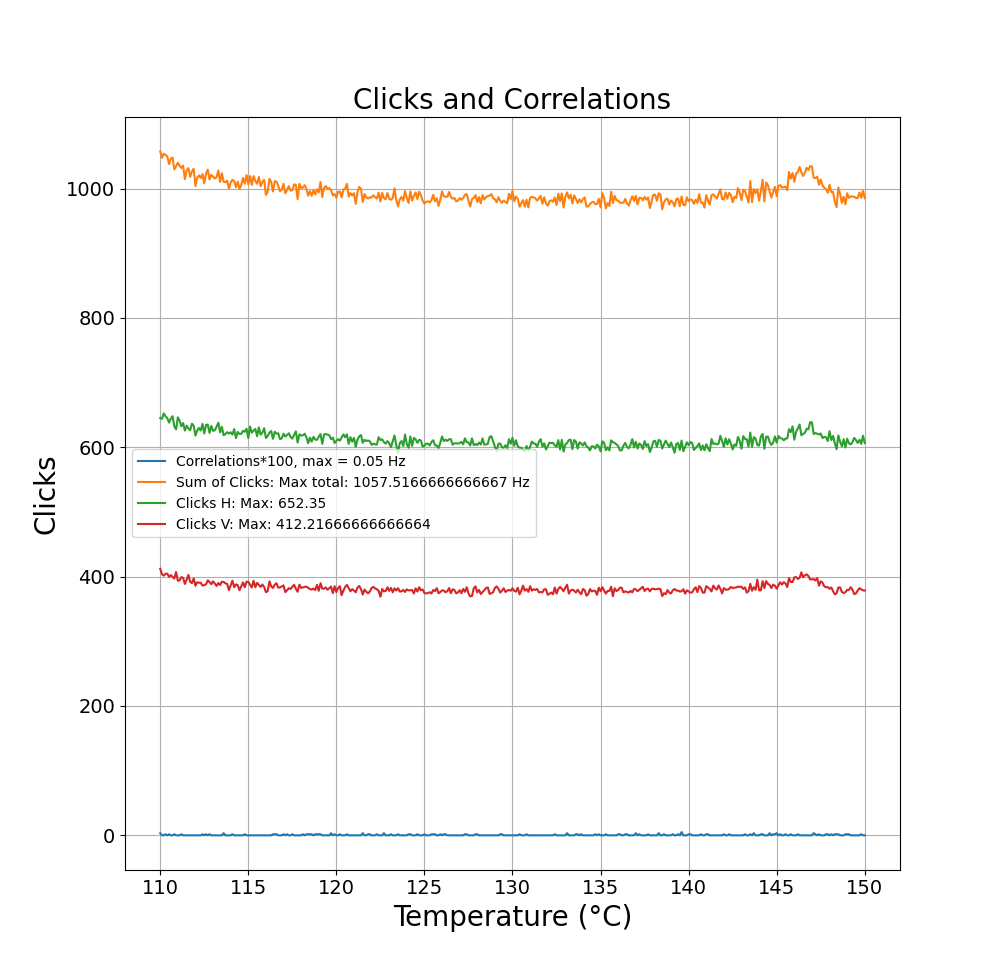
\includegraphics[width=2.9cm]{Not_Aligned_Scan.png}}\quad
	  \subfloat[][]{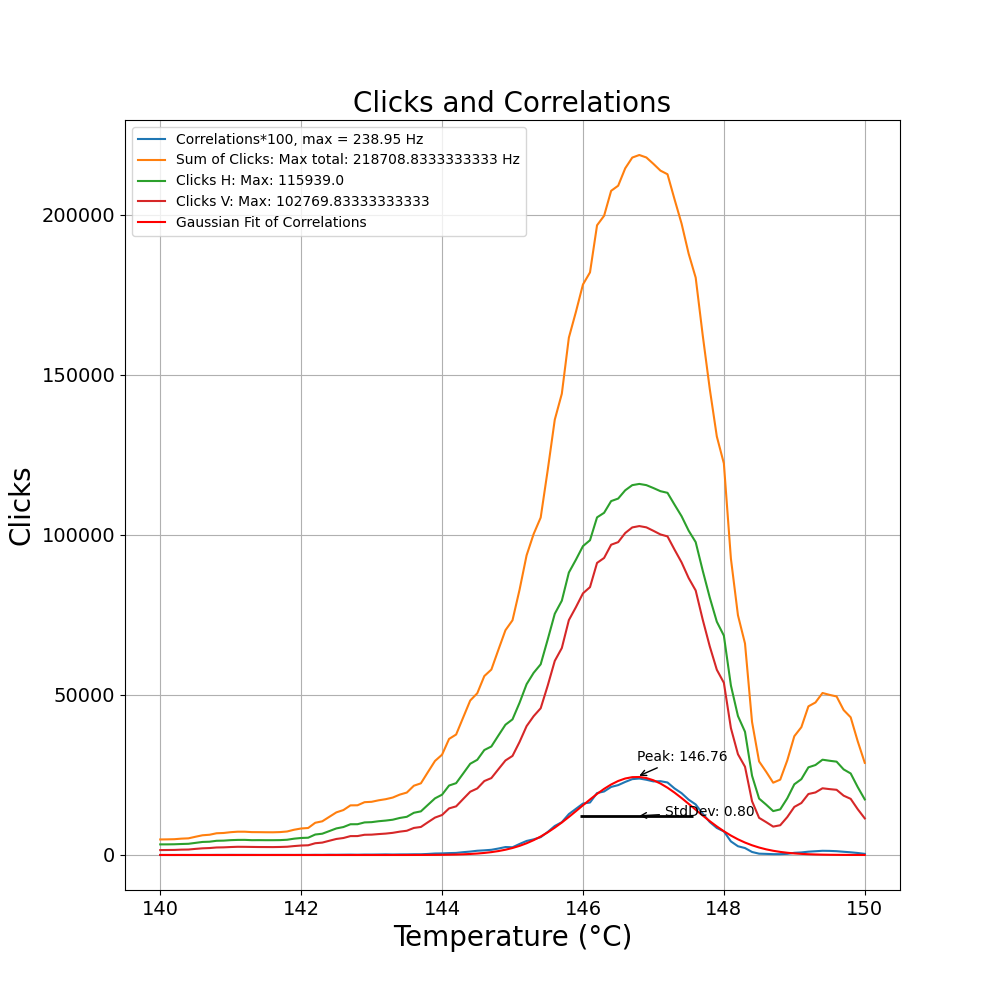
\includegraphics[width=2.9cm]{PMT_Grating_4.png}}\\
	  \subfloat[][]{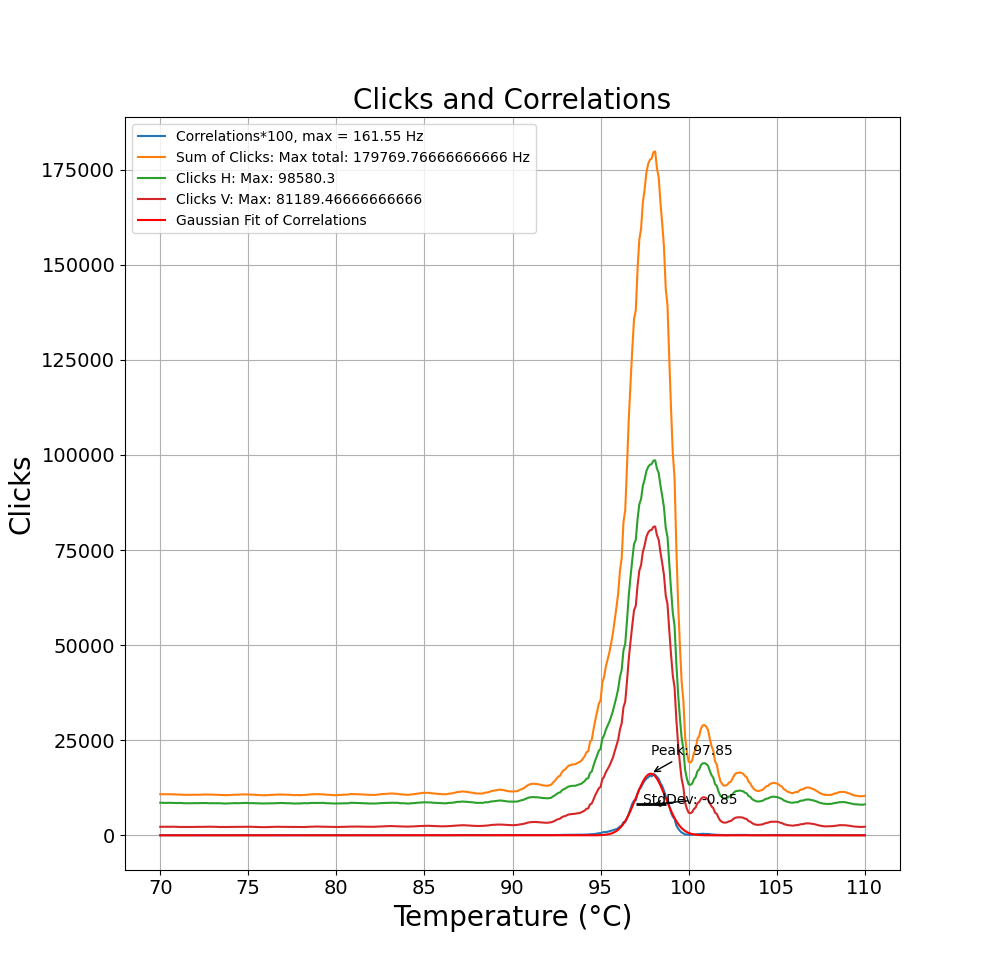
\includegraphics[width=2.9cm]{PMT_Grating_5.png}}\quad
	  \subfloat[][]{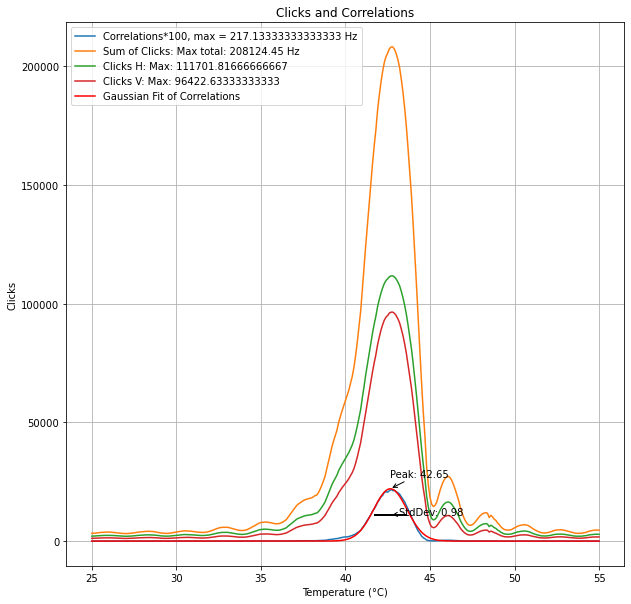
\includegraphics[width=2.9cm]{PMT_Grating_6.png}}\\
	  \label{fig:gratings}
	\end{figure}
\end{frame}

\subsection{Building a Sagnac Interferometer}
\usebackgroundtemplate{\includegraphics[width=\paperwidth,height=\paperheight]{SagnacWithSomeAddedColoursV3.png}}
\begin{frame}[t]
	\frametitle{Present state}
	\framesubtitle{Building a Sagnac Interferometer}
	  \pause
	\begin{figure}[!ht]
	  \centering
	  \includegraphics[width=9cm]{Type0Gratings.pdf}
	  \caption{\textcolor{white}{Specifications from the crystal manufacturer.\\\textit{Source: HC Photonics Corp.}}}
	\end{figure}
\end{frame}
\usebackgroundtemplate{}

\begin{frame}
	\frametitle{Present State}
	\framesubtitle{Current results}
	\begin{table}
		% Add measured numbers -- Quality of this model increases with the alignment.
		\begin{center}
			\caption{Current brightness estimation [$\frac{\text{Hz}}{\text{mWnm}}$]}
			\begin{tabular}[c|c|c]{|ll|l|}
				\hline
				\multicolumn{1}{|c}{\hfill\textbf{FMF}\hfill} &&
				\multicolumn{1}{c|}{\textbf{IJS}}\\
				\hline
				\multicolumn{1}{|c|}{\textbf{Type-II}} &
				\multicolumn{1}{c|}{\textbf{Type-0}} &
				\multicolumn{1}{c|}{\textbf{Type-II}}\\
				\hline
				7,8 $\times10^6$ \footnote{Linear setup} & 2,6 $\times 10^7 $  ^1 & 0,05 $\times 10^6$ \footnote{Sagnac interferometer}\\
				\hline
				\multicolumn{1}{|c}{\textbf{Bandwidth} [ nm ]} &\multicolumn{1}{c}{ } & \multicolumn{1}{c|}{ }\\
				\hline
				0,81 & 0,81 & 0,81\\
				\hline
			\end{tabular}
		\end{center}
	\end{table}
	% Overestimated for the "bad" detectors - One has to take into account the dead-time maybe so maybe no one is doing this correctly? :P
\end{frame}

\section{Outlook}
\begin{frame}{Outlook}
	\begin{itemize}
		\item Build the source
		\item Bell State Measurements %(CHSH)
		\item Entanglement swapping between FMF and IJS
		\item Free space link to IJS
		\item Fiber link to reactor
		\item Use Quantum Memory from IJS group
		\item SiQUID
			\begin{itemize}
				\item Building quantum network:
					\begin{enumerate}
						\item Experimental network
						\item Government network 
					\end{enumerate}
			\end{itemize}
	\end{itemize}
	% Entanglement swapping over short distance, IJS, Reactor with fibers, take one of the sources and do Entanglement swapping over long distances
\end{frame}

\addtocounter{framenumber}{-1}
\noPageNumber
\begin{frame}
	\frametitle{References}
	\tiny
	\bibliographystyle{IEEEtran}
	\bibliography{reference}
\end{frame}

\end{document}
